\appendix
\section{Numerical Experiments}

\begin{figure*}[t]
  \begin{center}
\subfigure[$p=10^{-3}$ and $q=p/20$]{
      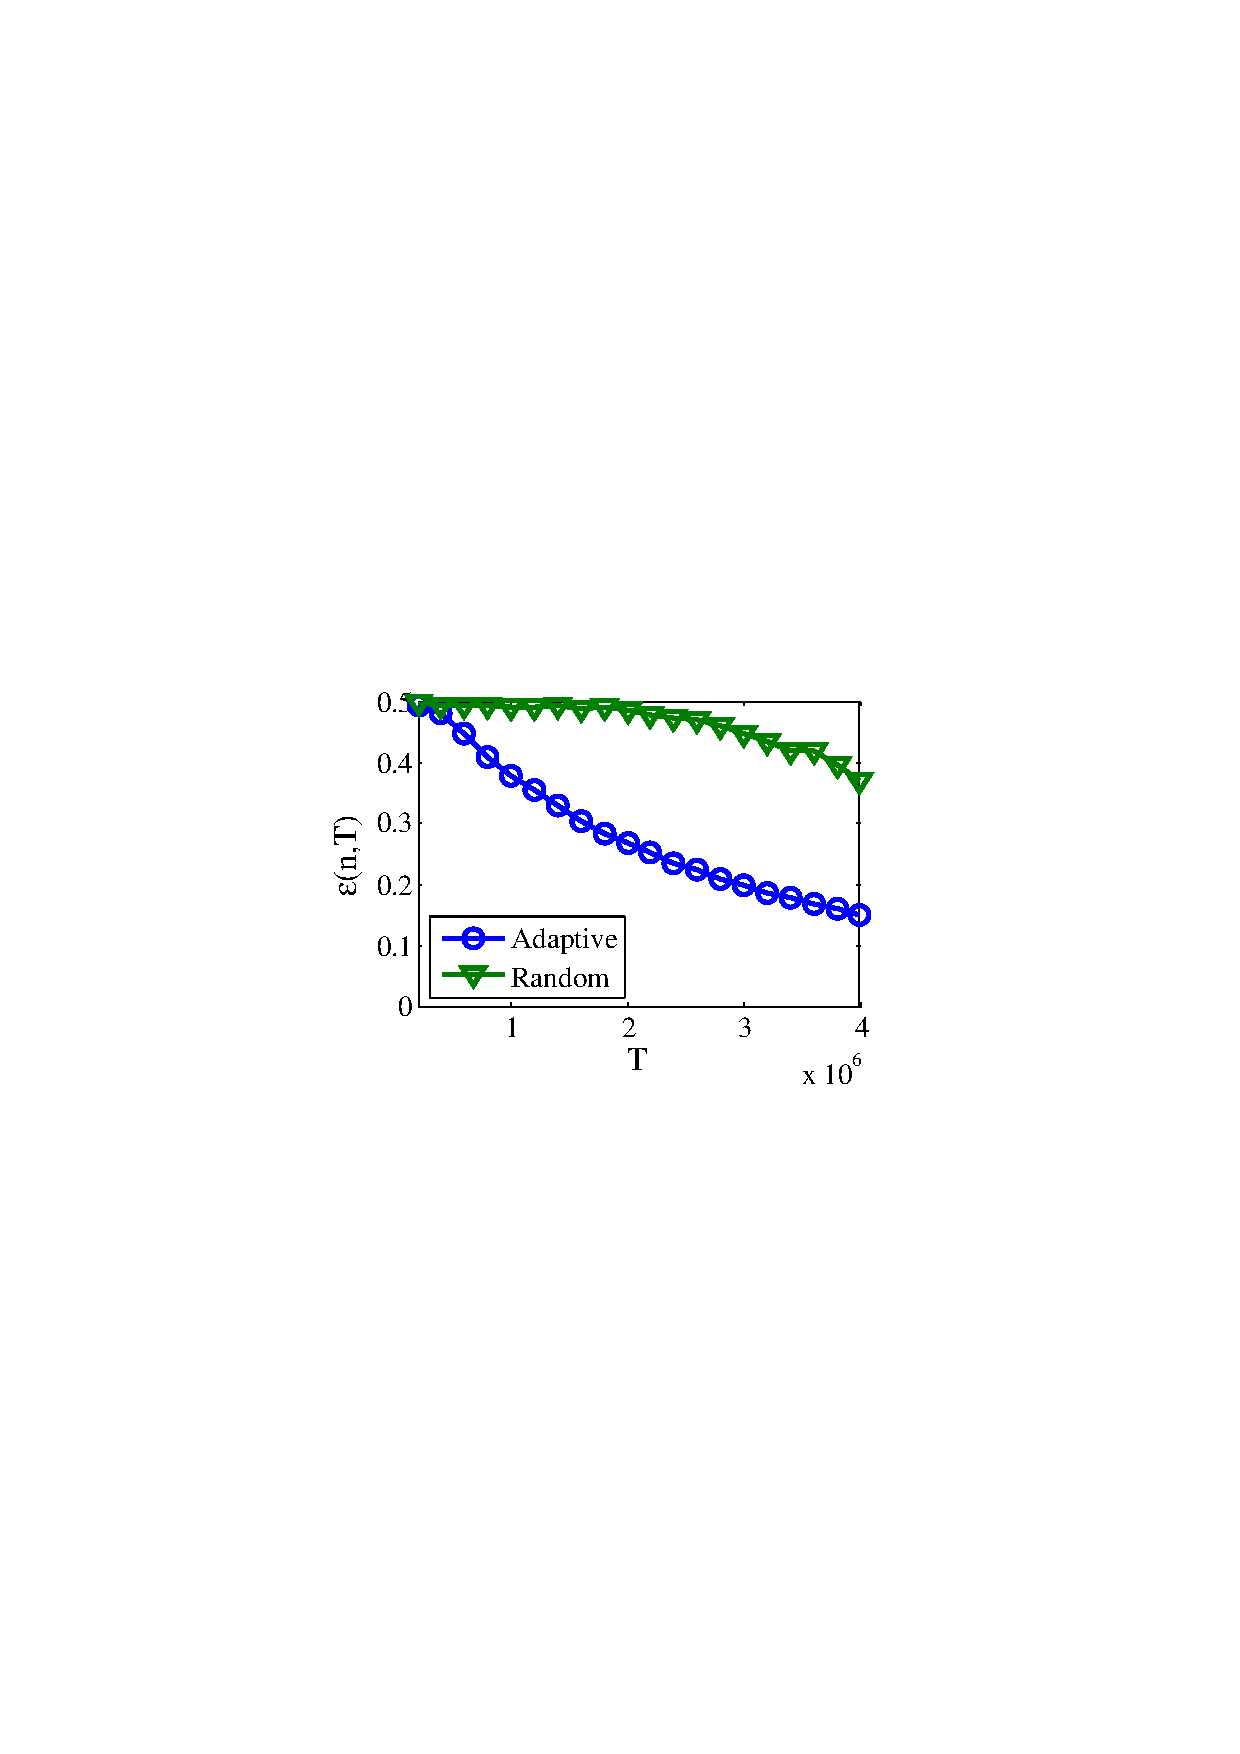
\includegraphics[width = 0.31\columnwidth]{fig/results1}} \label{fig:p1}
\subfigure[$p=10^{-2}$ and $q=p/2$]{
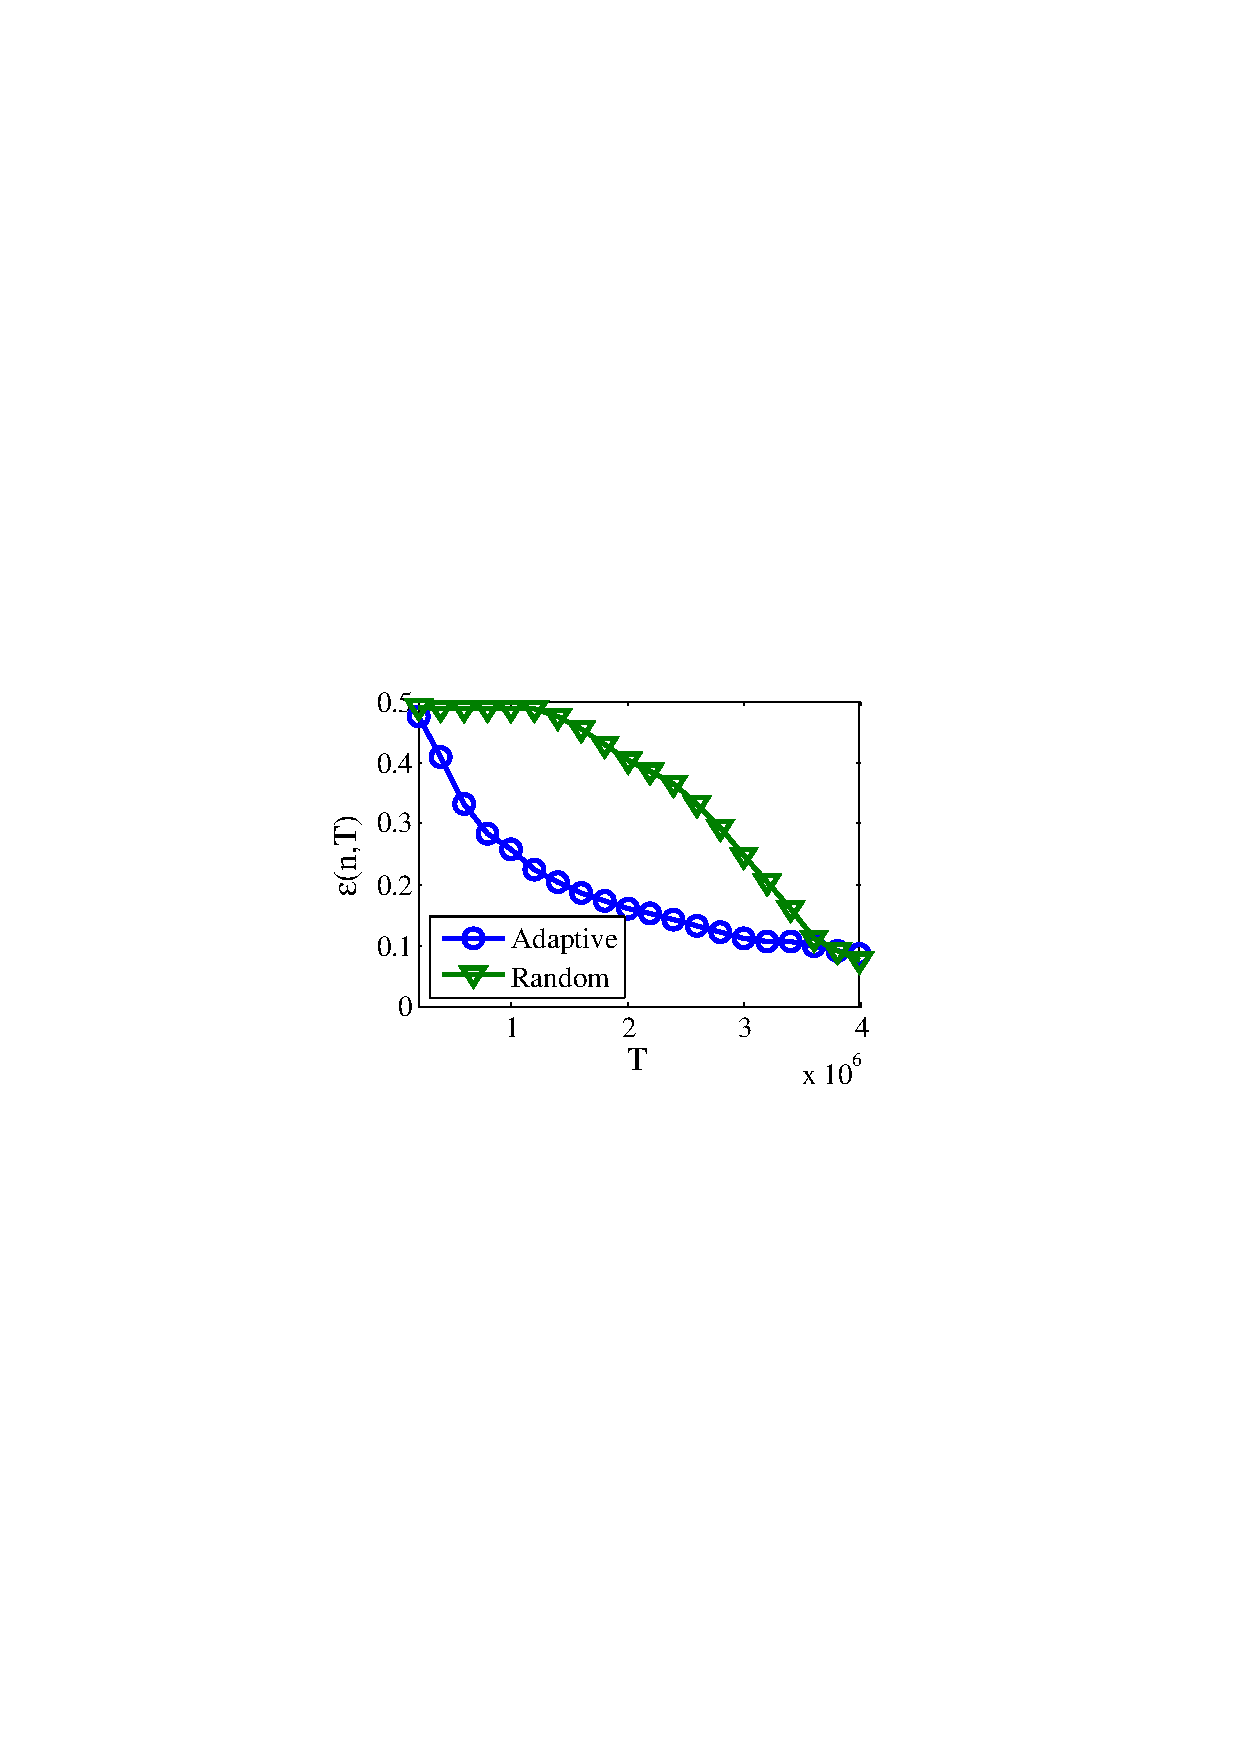
\includegraphics[width = 0.31\columnwidth]{fig/results2} \label{fig:p2}
}
\subfigure[$p=10^{-1}$ and $q=p/2$]{
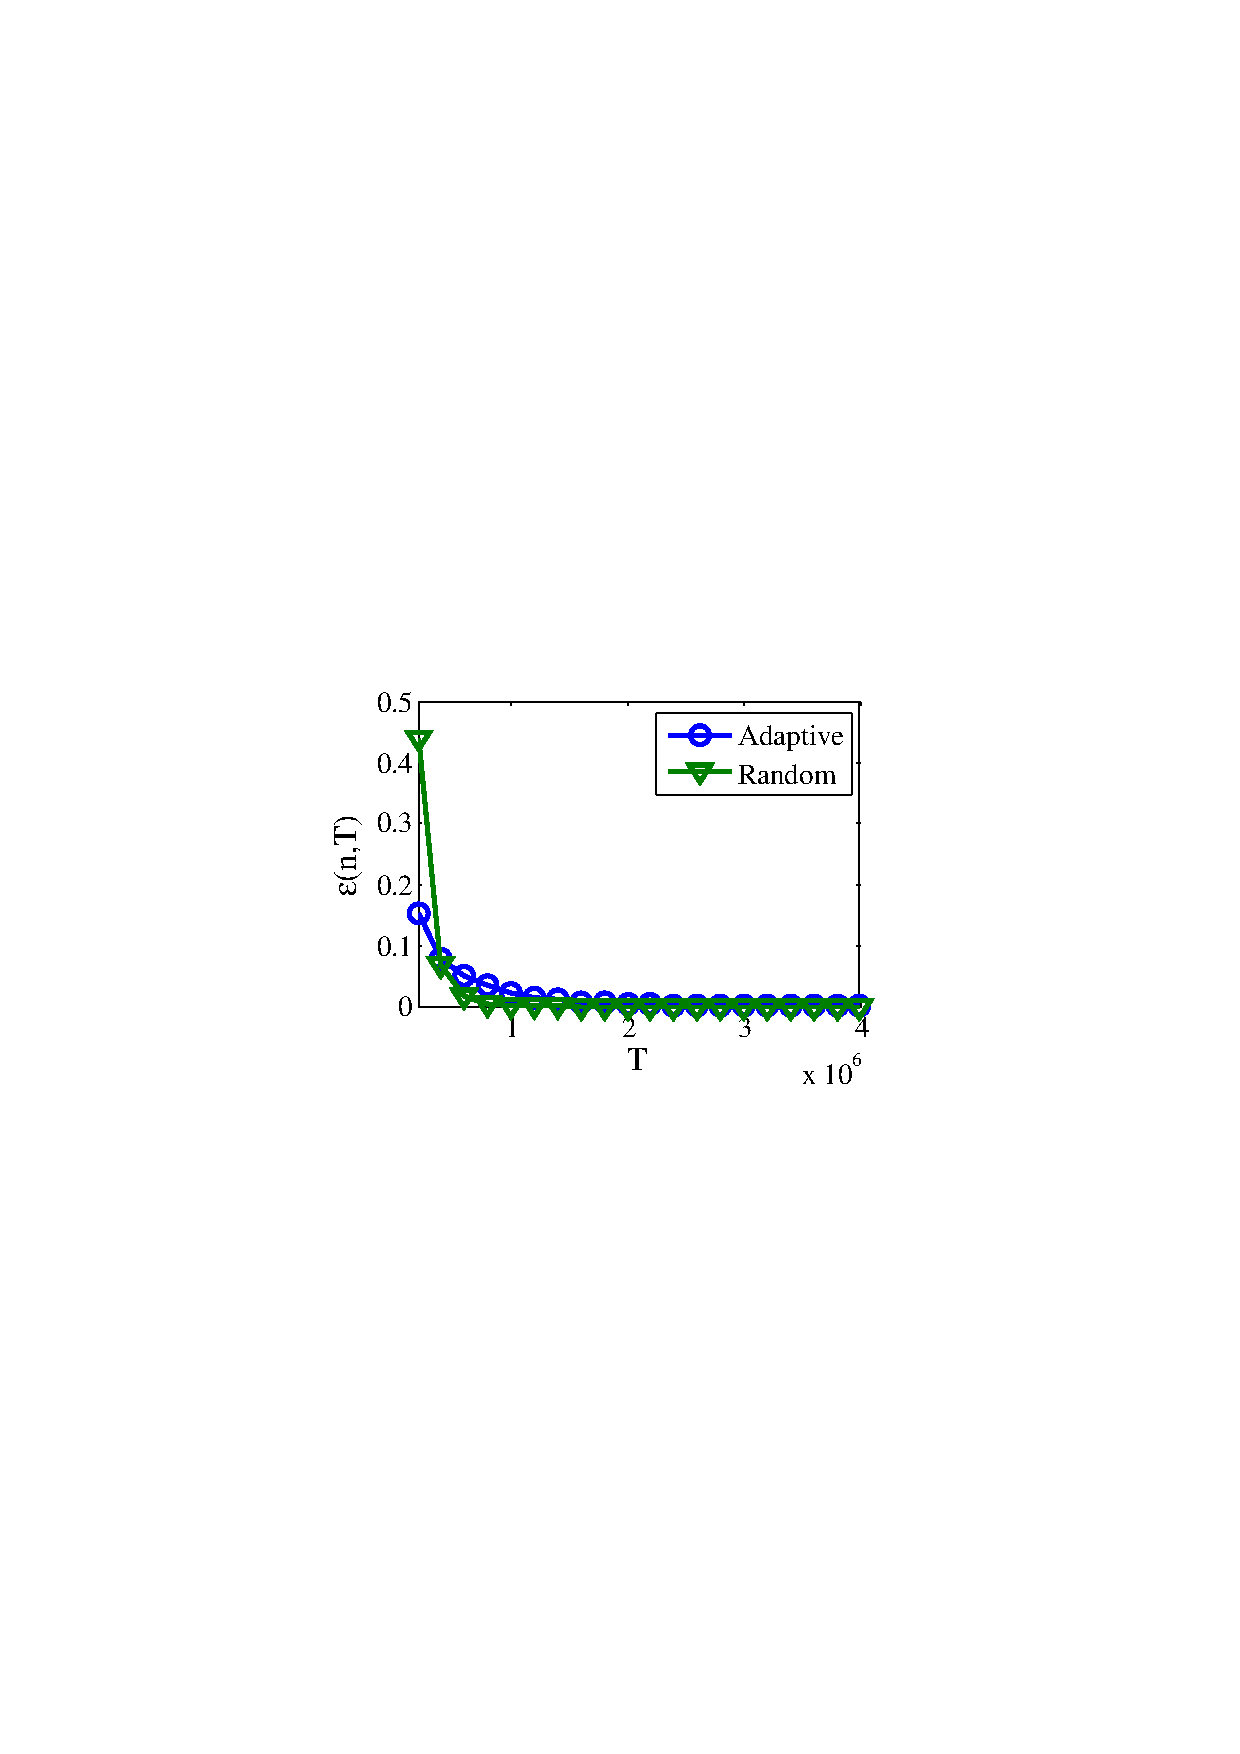
\includegraphics[width = 0.31\columnwidth]{fig/results3} \label{fig:p3}
}
    \caption{The average fraction of misclassified nodes under SP (URS-1 sampling strategy) and ASP.}
    \label{fig:numerical}
  \end{center}
\end{figure*}


In this appendix, using toy examples, we numerically compare the performance of SP and ASP. We consider a network of 4000 nodes and two communities ($K=2$) with equal sizes ($\alpha=0.5$). In Figure \ref{fig:numerical}, we plot the average fraction of misclassified nodes as a function of the observation budget $T$. We use the URS-1 sampling strategy (refer to as `Random' in the experiments). As expected, the adaptive sampling algorithm outperforms non-adaptive algorithms, and in general, the performance increases with $\frac{(p-q)^2}{p}\frac{T}{n}$. 

Under URS-2 sampling strategy, we know, from \cite{heimlicher2012community}, that the fraction of misclassified nodes cannot be less than $1/2$ when $\frac{(p-q)^2}{p+q}\frac{T}{n} < 1.$ For example, if $p=10^{-3}$ and $q=p/20$, $T = 2.326\times 10^{6}$ is the required budget to be able to design algorithms that perform better than simply assigning nodes to clusters randomly. This is consistent with the results of our numerical experiments: for non-adaptive sampling, the fraction of misclassified nodes is less than 0.5 if $T\ge 2.6\times 10^6$ (roughly). In this case, adaptive sampling provides much better performance: the fraction of misclassified nodes is less than 0.5 if $T\ge 4\times 10^5$. This good performance achieved even with a small budget can be explained by the fact that we use a fraction $T/5$ of the budget on a small fraction of nodes ($n/5 \log n$ nodes) to identify kernels. The phase transition then occurs when $\frac{(p-q)^2}{p+q}\log n \frac{T}{n} < 1$, i.e., when $T=3\times 10^5.$ 




%%% Local Variables: 
%%% mode: latex
%%% TeX-master: "clustering_colt"
%%% End: 

